\documentclass[tikz,border=4pt]{standalone}
\usepackage[T1]{fontenc}
\usepackage{lmodern}
\usepackage{amsmath}
% Shared TikZ style for the report figures.
% Colours follow the Okabe-Ito palette, which stays distinguishable under the
% common forms of colour-vision deficiency. Every colour-coded element also
% carries a text label, so no figure depends on colour alone.
\usetikzlibrary{arrows.meta,positioning,fit,calc,backgrounds,decorations.pathreplacing,shapes.geometric}

\definecolor{oiOrange}{HTML}{E69F00}
\definecolor{oiSky}{HTML}{56B4E9}
\definecolor{oiGreen}{HTML}{009E73}
\definecolor{oiYellow}{HTML}{F0E442}
\definecolor{oiBlue}{HTML}{0072B2}
\definecolor{oiVerm}{HTML}{D55E00}
\definecolor{oiPurple}{HTML}{CC79A7}
\definecolor{oiGray}{HTML}{6E6E6E}

\colorlet{corTreino}{oiBlue!22}
\colorlet{corValid}{oiGreen!30}
\colorlet{corTeste}{oiOrange!45}
\colorlet{corControle}{oiPurple!35}

\tikzset{
  >=Stealth,
  bloco/.style={draw=black!70, rounded corners=1.5pt, minimum height=0.62cm,
    inner sep=2pt, font=\sffamily\fsz, align=center},
  treino/.style={bloco, fill=corTreino},
  valid/.style={bloco, fill=corValid},
  teste/.style={bloco, fill=corTeste, thick},
  etapa/.style={draw=black!70, rounded corners=3pt, fill=black!4,
    text width=4.3cm, align=center, inner sep=4pt, font=\sffamily\fsz},
  nota/.style={font=\sffamily\fsz, align=left, text=black!80},
  titulo/.style={font=\sffamily\fst\bfseries, anchor=west},
  seta/.style={->, thick, black!70},
  regiao/.style={draw=black!50, dashed, rounded corners=4pt},
}

% Absolute font sizes, so a figure looks the same standalone (10 pt class) and
% inside the 11 pt report.
\providecommand{\fsx}{\fontsize{5.5}{6.5}\selectfont}
\providecommand{\fsz}{\fontsize{7}{8.5}\selectfont}
\providecommand{\fst}{\fontsize{9}{11}\selectfont}

\begin{document}
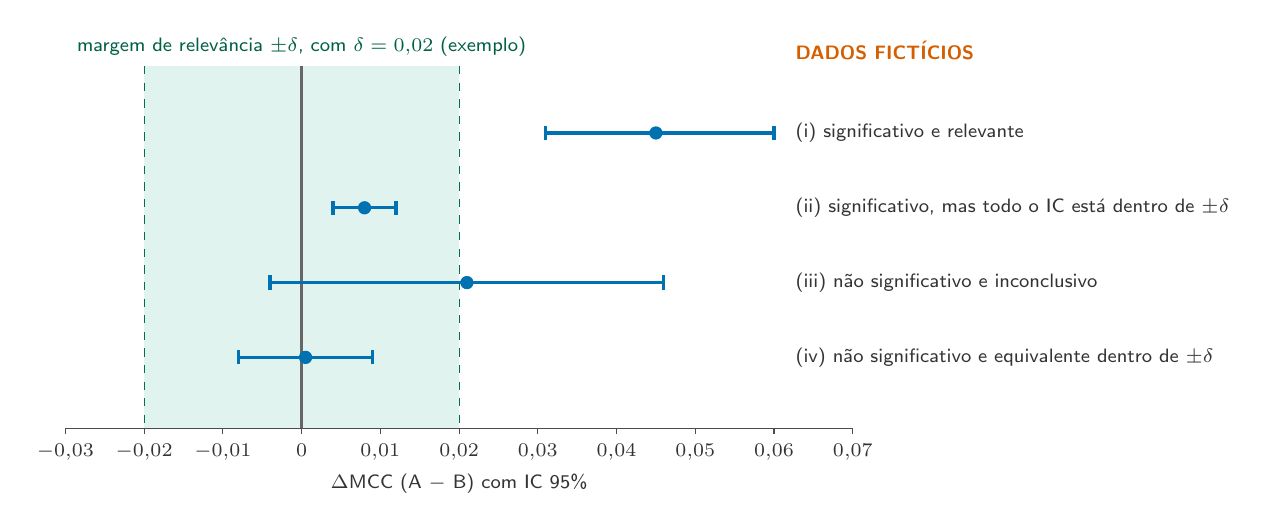
\begin{tikzpicture}[x=100cm]
  % x axis: Delta MCC from -0.03 to 0.07 (1 unit = 100 cm, so 0.01 = 1 cm)
  \fill[oiGreen!12] (-0.02,0.35) rectangle (0.02,-4.25);
  \draw[black!70] (-0.03,-4.25) -- (0.07,-4.25);
  \foreach \v/\t in {-0.03/$-0{,}03$,-0.02/$-0{,}02$,-0.01/$-0{,}01$,0/$0$,0.01/$0{,}01$,0.02/$0{,}02$,0.03/$0{,}03$,0.04/$0{,}04$,0.05/$0{,}05$,0.06/$0{,}06$,0.07/$0{,}07$} {
    \draw[black!70] (\v,-4.25) -- (\v,-4.32);
    \node[nota, anchor=north] at (\v,-4.32) {\t};
  }
  \node[nota] at (0.02,-4.95) {$\Delta$MCC (A $-$ B) com IC 95\%};
  \draw[black!60, thick] (0,0.35) -- (0,-4.25);
  \draw[oiGreen!70!black, dashed] (-0.02,0.35) -- (-0.02,-4.25);
  \draw[oiGreen!70!black, dashed] (0.02,0.35) -- (0.02,-4.25);
  \node[nota, text=oiGreen!60!black, anchor=south] at (0,0.35) {margem de relevância $\pm\delta$, com $\delta = 0{,}02$ (exemplo)};
  \node[font=\sffamily\fsz\bfseries, text=oiVerm, anchor=west] at (0.0615,0.55) {DADOS FICTÍCIOS};
  % scenarios: label, estimate, low, high
  \foreach \i/\est/\lo/\hi/\rot in {
      1/0.045/0.031/0.060/{(i) significativo e relevante},
      2/0.008/0.004/0.012/{(ii) significativo, mas todo o IC está dentro de $\pm\delta$},
      3/0.021/-0.004/0.046/{(iii) não significativo e inconclusivo},
      4/0.0005/-0.008/0.009/{(iv) não significativo e equivalente dentro de $\pm\delta$}} {
    \pgfmathsetmacro\y{-0.95*\i+0.45}
    \draw[very thick, oiBlue] (\lo,\y) -- (\hi,\y);
    \draw[very thick, oiBlue] (\lo,\y-0.09) -- (\lo,\y+0.09);
    \draw[very thick, oiBlue] (\hi,\y-0.09) -- (\hi,\y+0.09);
    \fill[oiBlue] (\est,\y) circle (2.4pt);
    \node[nota, anchor=west] at (0.0615,\y) {\rot};
  }
\end{tikzpicture}
\end{document}
